% !TeX encoding = UTF-8
% !TeX program = xelatex
\iffalse
########################
Project Name:
    The LaTeX cn/en template for MUST Thesis 
Github:
    https://github.com/iihciyekub/MUST-Thesis
User's Guide:
    https://iihciyekub.github.io/must-thesis-manual
Overleaf texAide (Chrome Extension):
    https://chrome.google.com/webstore/detail/overleaf-s2tbib2bbl/icekiliecbhnockmfkehoebbkmhmapmo?hl=zh-CN

Author: Yongjian.Li (LastUpdate: Feb 21, 2025 at 12:23:13)
########################
\fi

\documentclass[writingLanguage=chinese, % 中文模板
    addPageTitle=on,  % on/off 添加扉頁
    addDeclaration=on, % on/off 添加原創聲明
    addMUSTlog=off, % on/off 添加校徽水印
    addFigTOC=on, % on/off 添加圖目錄  
    addTabTOC=on, % on/off 添加表目錄
    refIndent=off, % on/off 修改參考文獻條目縮進
    printMod=off, % on/off 設置奇偶數邊距對稱紙質打印模式
]{.def/must}

\usepackage{markdown}
\usepackage{tikz-uml}
\usepackage{pdflscape}

% 論文基本信息,必填不能刪除
\def\school              {Macau University of Science and Technology}
\def\cnTitle            {基於虛幻引擎的遊戲手機與開發}
\def\cnShortTitle       {\cnTitle} % 頁眉顯示的中文論文短題目
\def\enTitle            {Game Design and Development Based on Unreal Engine}
\def\enShortTitle       {\enTitle} % 頁眉顯示的英文論文短題目
\def\Name               {時韋豪} % 作者名稱
\def\StudentNo          {2230009444} % 學號
\def\Faculty 	        {人文藝術學院} % 所在學院
\def\Program 	        {互動媒體與藝術學院} % 學位名稱
\def\Major              {遊戲設計} % 專業名稱
\def\Supervisor	        {黃鶯} % 指導老師
\def\DateofWriting		{\datea\today} % 設置論文寫作完成時間
\def\DateofDeclaration	{2024/04/21} % 設置論文原創聲明時間
\def\DateofSignature	{2024/04/21} % 設置簽署論文原創聲明的時間
\def\PublicAfterYears   {5} % 設置論文幾年後公開
\def\mySign             {Fig/mySign.png} %使用帶透明通道的 png 照片(推薦)
\def\supervisorSign     {Fig/supervisorSign.png} %使用帶透明通道的png照片






\begin{document}

% 導入中文摘要
\input{content/a_cn_abs}

% 導入英文摘要
\input{content/a_en_abs}


% 生成目錄,包含圖與表
\addtableofcontents


% 導入正文第一章, [自行添加其它章節 tex 文件, 可自定義路徑與文件名]
\chapter{緒論}
\section{開發背景}
\section{開發目的與意義}
\section{創新點和特色}
\citep{abdoh2019} 引用
\subsection{論文寫作依據}
正文部位写

\chapter{遊戲總體設計}
\section{世界觀與故事背景}
\section{玩法核心機制和體驗目標}
\citep{abdoh2019} 引用
\subsection{論文寫作依據}
正文部位写
\iffalse
########################
\subsubsection{概述}
\subsubsection{設計目標}
\paragraph{\Large\bfseries 面向玩家的目標}
\begin{markdown}

\end{markdown}
\paragraph{\Large\bfseries 面向藝術家的目標}
\begin{markdown}

\end{markdown}
\paragraph{\Large\bfseries 面向程序員的目標}
\begin{markdown}

\end{markdown}
\paragraph{\Large\bfseries 面向遊戲設計師的目標}
\begin{markdown}

\end{markdown}
\subsubsection{UML圖繪製}

########################
圖片模版
\begin{figure}[h]
    \centering
      \fbox{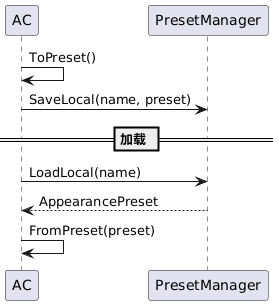
\includegraphics[width=0.34\textwidth]{Fig/UML/Chapter3/3_1_1.png}}
    \caption{玩家預設和保存外觀時間序列圖}
    \label{fig:uml-player}
\end{figure}

橫向大圖模版
\begin{landscape}
\begin{figure}[htbp]
  \centering
  \vspace*{\fill} 
      \fbox{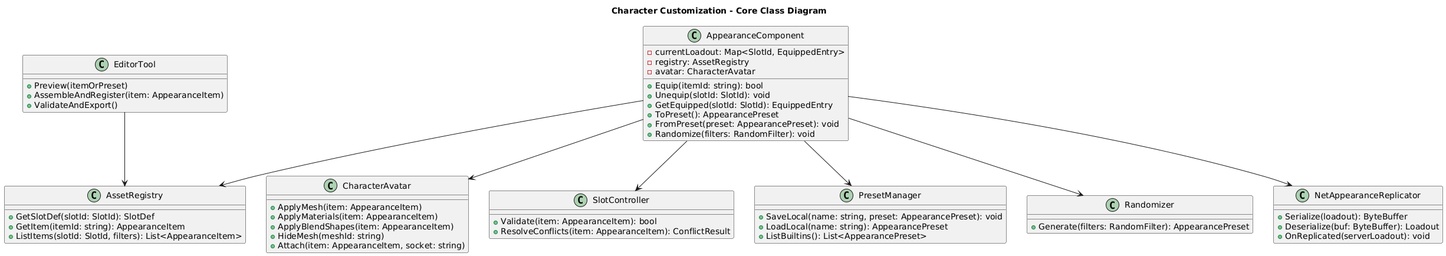
\includegraphics[width=1.5\textwidth]{Fig/UML/Chapter3/3_1_2.png}}
    \caption{自定義外觀系統類圖}
\end{figure}
\end{landscape}

########################
\fi

\chapter{系統架構設計}
\section{玩家角色系統}
\subsection{自定義外觀系統}
\subsubsection{概述}
遊戲中可能會有非常多的不同類型、不同性格的角色，以及能讓玩家去自訂個性化自己的角色。如何拆解這個角色以供玩家自訂是非常必要的，我將角色拆解為無數個部分，以讓玩家和美術能組合出無數個不同風格的角色組合。
\subsubsection{設計目標}

\paragraph{\Large\bfseries 面向玩家的目標}
\begin{markdown}
- 自由定制角色外觀
    - 可以配置角色頭部頂部裝飾（帽子、髮飾）
    - 可以配置角色眉毛形態
    - 可以配置角色眼睛形態
    - 可以配置角色鬍鬚形態
    - 可以配置角色嘴部形態
    - 可以配置角色上身外觀（服裝、盔甲）
    - 可以配置角色手部外觀（手套、飾品）
    - 可以配置角色下身外觀（褲裝、裙裝）
    - 可以配置角色腳部外觀（鞋靴）
- 保存與使用外觀
    - 可以保存自定義外觀預設
    - 可以載入美術設計好的外觀預設
    - 可以生成或使用隨機外觀預設
- 互動體驗
    - 外觀變化即時顯示於角色模型
    - 可在角色介面中預覽與旋轉模型
\end{markdown}

\paragraph{\Large\bfseries 面向藝術家的目標}
\begin{markdown}
- 資產製作
    - 美術師可以產出不同部位的美術資產（頭部、身體、手部、腳部）
    - 支援多種貼圖類型（顏色、法線、金屬度）
    - 支援多層材質疊加效果
- 資產管理
    - 可使用工具介面直接導入與註冊新資產
    - 可視化組裝角色各部位，快速預覽搭配效果
    - 在不修改程式碼的情況下添加新外觀組件
\end{markdown}

\paragraph{\Large\bfseries 面向程序員的目標}
\begin{markdown}
- 系統結構
    - 實現基礎外觀組件系統
    - 建立統一的槽位（Slot）機制：頭部、身體、手部、腳部等
    - 支援多玩家同步外觀資料
- 擴充與維護
    - 模組化程式設計，允許添加新的裝備槽
    - 透過資料驅動方式載入外觀配置
    - 提供 API 介面供 UI 與工具使用
\end{markdown}

\paragraph{\Large\bfseries 面向遊戲設計師的目標}
\begin{markdown}
- 體驗設計
    - 確保玩家在創角或遊戲中能自由改變外觀
    - 外觀系統需與遊戲進程、任務或貨幣系統結合
- 平衡與獎勵
    - 透過任務或活動解鎖外觀部件
    - 控制稀有度與可獲取條件
    - 可配置角色外觀在特定場景的限制（如職業、陣營）
\end{markdown}  


\subsubsection{UML圖繪製}
\begin{figure}[h]
    \centering
      \fbox{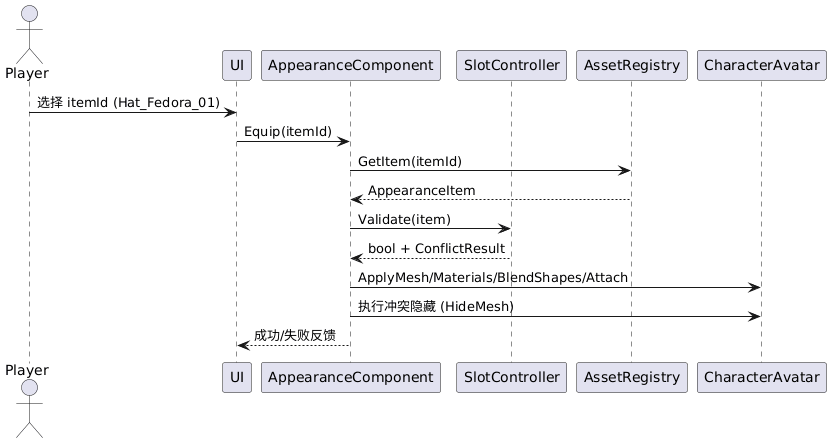
\includegraphics[width=1\textwidth]{Fig/UML/Chapter3/3_1_0.png}}
    \caption{玩家自定義外觀時間序列圖}
    \label{fig:uml-player}
\end{figure}

\begin{figure}[h]
    \centering
      \fbox{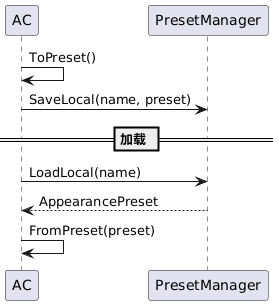
\includegraphics[width=0.34\textwidth]{Fig/UML/Chapter3/3_1_1.png}}
    \caption{玩家預設和保存外觀時間序列圖}
    \label{fig:uml-player}
\end{figure}

\begin{landscape}
\begin{figure}[htbp]
  \centering
  \vspace*{\fill} 
      \fbox{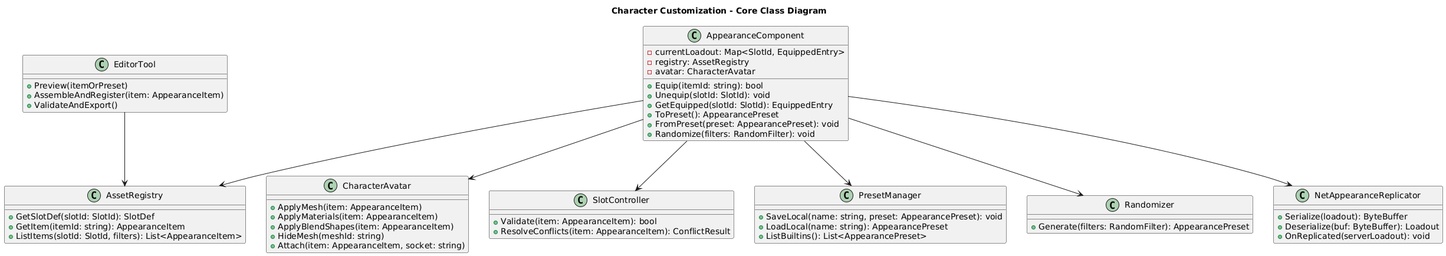
\includegraphics[width=1.5\textwidth]{Fig/UML/Chapter3/3_1_2.png}}
    \caption{自定義外觀系統類圖}
\end{figure}
\end{landscape}


\subsection{屬性數值系統}

\subsubsection{概述}
玩家自身維持著一個動態屬性數值系統，例如各部位的血量、耐力數值、飽食度數值、負重數值、水分含量數值、情緒狀態等不同的資料模組。為此，建立一個可擴展、可插拔、模組化的資料系統顯得非常必要。
\subsubsection{設計目標}
\paragraph{\Large\bfseries 面向玩家的目標}
\begin{markdown}
- 玩家需要維護自身各個部位的血量健康情況
  - 頭部
    - 受到一定傷害後的反應
    - 受到大量傷害後的反應
    - 健康值為 0 時的反應
  - 膝膝
    - 受到一定傷害後的反應
    - 受到大量傷害後的反應
    - 健康值為 0 時的反應
  - 胸部
    - 受到一定傷害後的反應
    - 受到大量傷害後的反應
    - 健康值為 0 時的反應
  - 腿部
    - 受到一定傷害後的反應
    - 受到大量傷害後的反應
    - 健康值為 0 時的反應
  - 胃部
    - 受到一定傷害後的反應
    - 受到大量傷害後的反應
    - 健康值為 0 時的反應
- 玩家需要維護自身的飽食度
  - 當前飽食度數值
  - 最大飽食度數值
  - 飽食度數值離散變化
    - 使用某種行為／動作消耗
      - 揮砍
      - 拉弓
      - 開槍
      - 疾跑
      - 工作
  - 飽食度數值線性變化
    - 隨時間自然消耗
      - 基礎角色自然消耗
      - 負重數據附加
    - 使用某種物品後隨一定時間消耗
  - 定義飽食度狀態
    - 吃撐
    - 滿足
    - 正常
    - 微飢
    - 飢餓
    - 極度飢餓
- 玩家需要維護自身的水分
  - 當前水分含量
  - 最大水分含量
  - 水分含量離散變化
    - 執行行為或動作消耗
      - 疾跑
      - 吃特定食物
  - 水分含量線性變化
    - 隨時間自然消耗
      - 角色基礎自然消耗
      - 自身負重消耗
    - 使用某種物品後隨一定時間消耗
  - 定義水分含量狀態
    - 正常
    - 缺水
    - 脫水
- 玩家需有耐力值管理能力
  - 最大耐力值
  - 當前耐力值
  - 耐力值離散變化
  - 耐力值線性變化
  - 定義當前耐力狀態
    - 充沛
    - 疲勞
    - 無力
  - 數值變化與負重息息相關
- 玩家能管理自己的負重能力
  - 最大負重值
  - 當前負重值
  - 變化負重數值
  - 定義負重狀態
    - 輕鬆
    - 微重
    - 正好應對
    - 超重
- 玩家擁有情緒狀態記錄 
  - 詞條列表（見下方表格\ref{tab:emotion_state}）
  - 不同情緒狀態的反應
  - 變化情緒狀態詞條的能力
- 玩家製造物品速度

\end{markdown}
\paragraph{\Large\bfseries 面向藝術家的目標}
\begin{markdown}
- 數值系統的 UI 呈現
\end{markdown}
\paragraph{\Large\bfseries 面向程序員的目標}
\begin{markdown}
- 數據分層
- 統一修改入口：所有改動走 ApplyInstant / ApplyOverTime / AddModifier / RemoveModifier，外部系統（武器、道具、環境）不直接改變數值。
- 事件驅動：OnStatChanged、OnBodyPartWounded、OnDeath
- 代碼結構：Tick 中按時間推進（SimTime），模擬體溫、出血、感染、耐力恢復等。
- 網絡：服務端權威；FastArray 複製高頻更新數據，客戶端本地 UI 訂閱「聚合值」。
- 存檔：序列化全局屬性、各部位狀態，支持 OverTime 與 Modifiers。
\end{markdown}
\paragraph{\Large\bfseries 面向遊戲設計師的目標}
\begin{markdown}
- 數值由 CSV 表格驅動和配置
\end{markdown}

\begin{table}[htbp]
\centering
\caption{角色情緒狀態表}
\label{tab:emotion_state}
\begin{tabularx}{\textwidth}{c|X|X}
\toprule
\textbf{詞條名稱} & \textbf{觸發條件} & \textbf{效果} \\
\midrule
平靜 & 一般正常狀態 & 無效果 \\
冷靜 & 使用某種物品後，如煙等 & 人物動作變快 \\
愉悅 & 使用某種物品後，如花卉嗅覺等 & 血量恢復速度提高，體力恢復速度提高 \\
興奮 & 使用某種物品後，如可卡因等 & 代謝速度加快，人物動作變快，體力恢復速度提高 \\
不安 & 降低一定血量後，使用成癮物品後 & 代謝速度變快，疲勞速度變快 \\
厭惡 & 降低大量血量後，吃壞東西等 & 損失飽食度，代謝速度變慢，人物動作及恢復速度變慢 \\
焦慮 & 降低大量血量後，使用成癮物品後 & 血量恢復速度變慢 \\
\bottomrule
\end{tabularx}
\end{table}

\subsubsection{UML圖繪製}

\begin{landscape}
\begin{figure}[htbp]
  \centering
  \vspace*{\fill} 
      \fbox{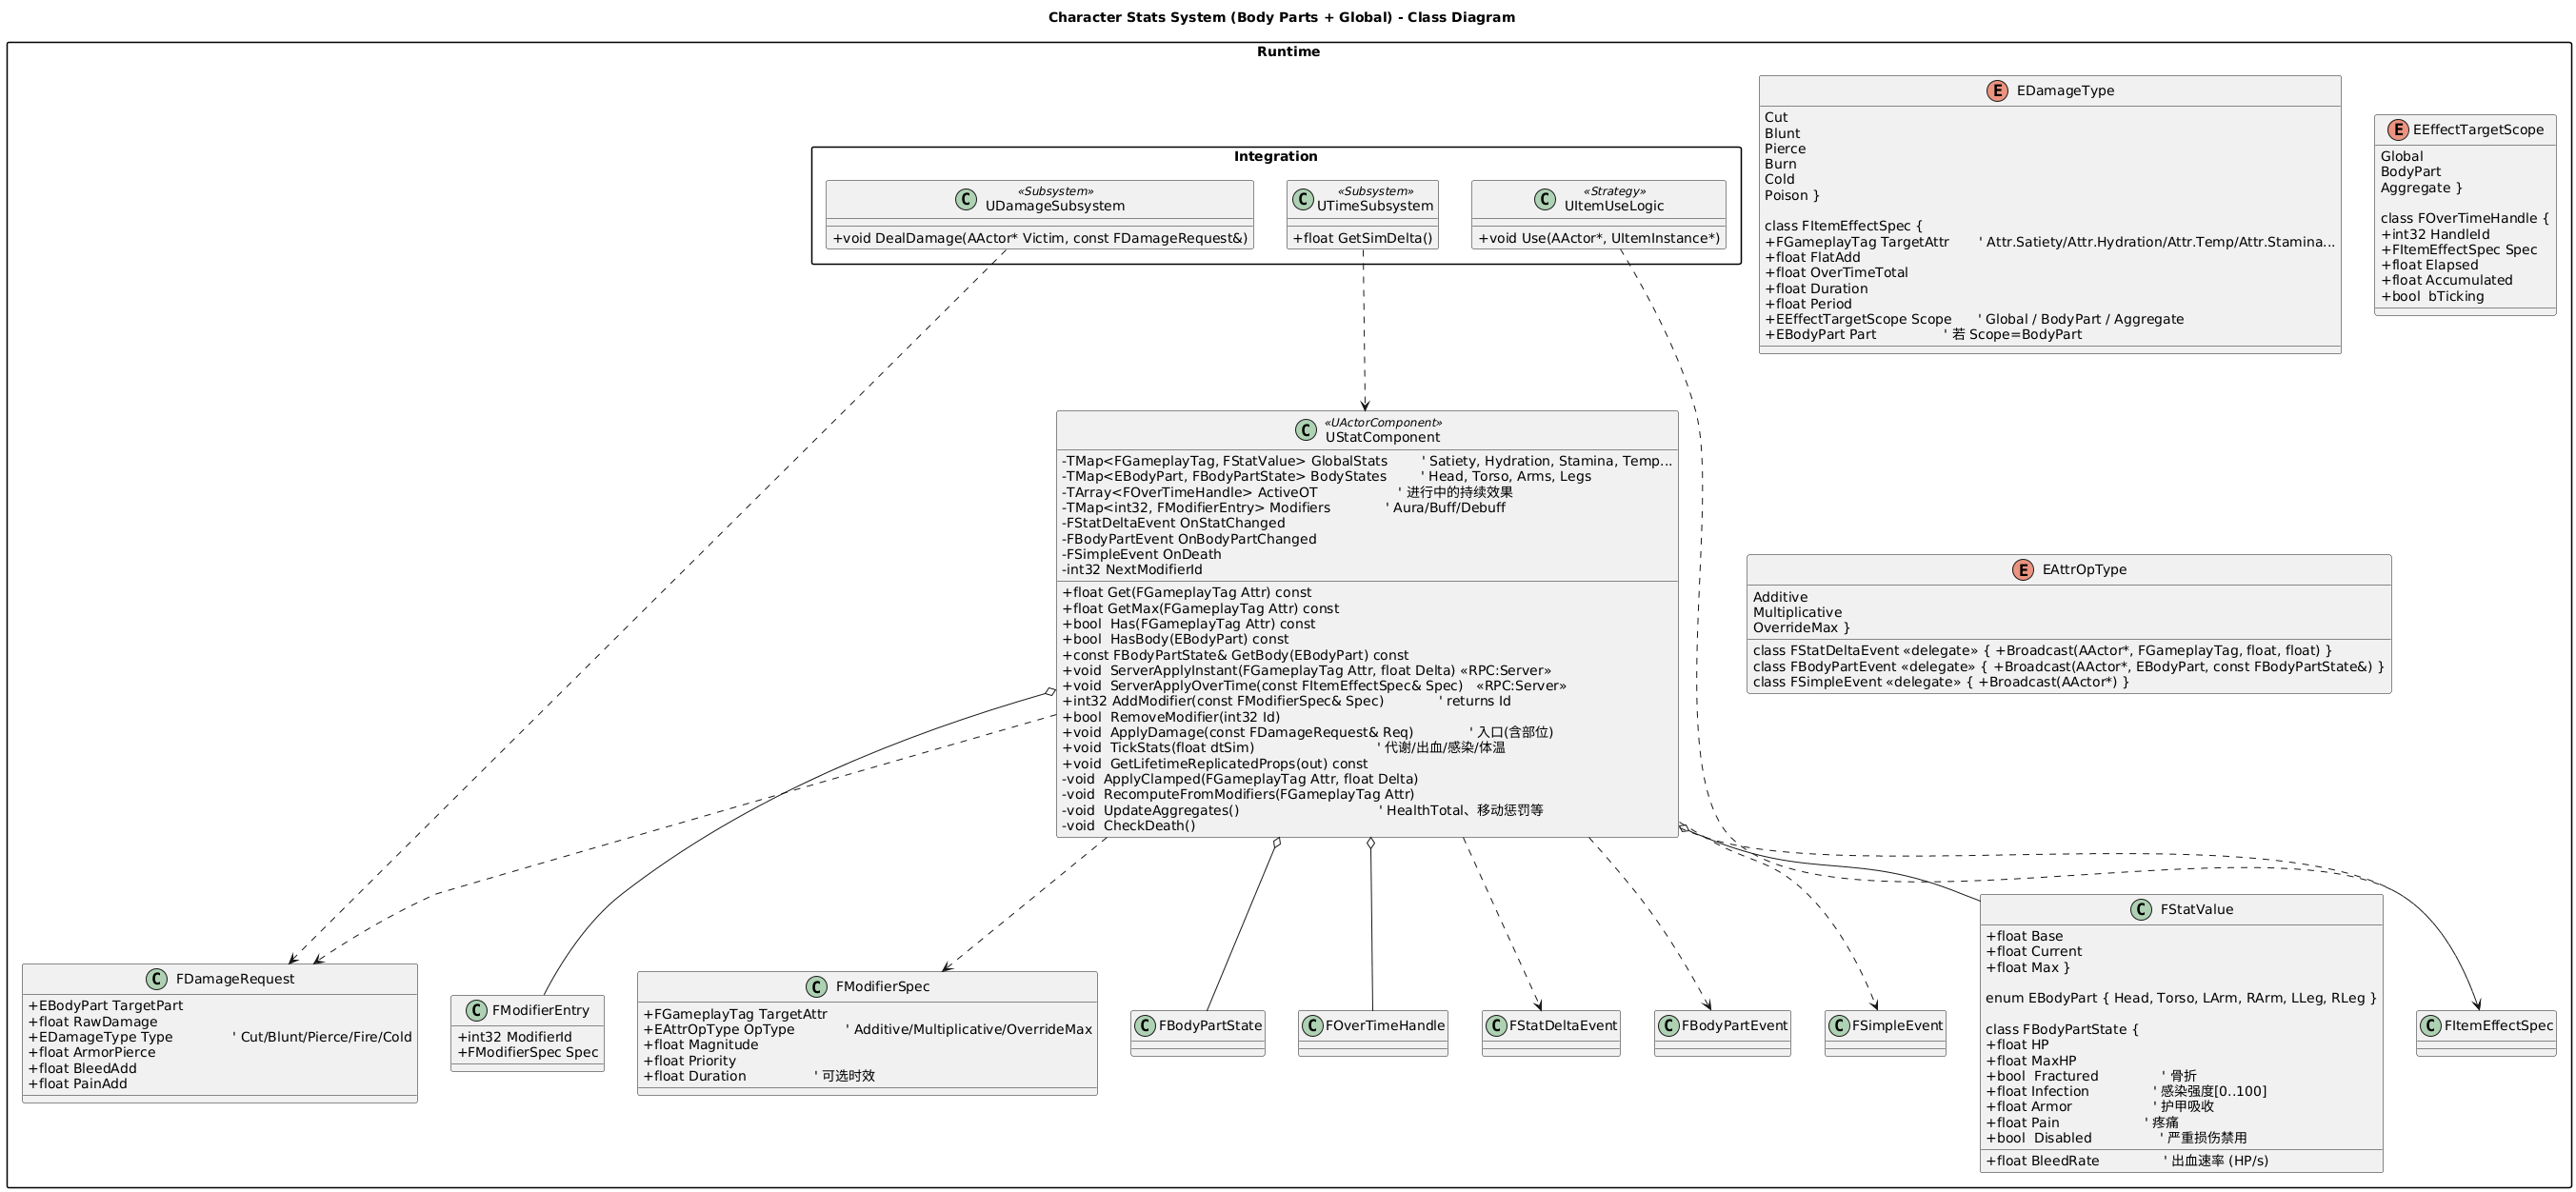
\includegraphics[width=1.6\textwidth]{Fig/UML/Chapter3/3_2_1.png}}
    \caption{角色屬性數值系統類圖}
\end{figure}
\end{landscape}


\subsection{背包系統}

\subsubsection{概述}
玩家在場景中會探索出各種物品；如何儲存與管理物品是遊戲機制中非常關鍵的一部分。這裡我嘗試製作類似《逃離塔科夫》的背包管理系統，即以「物品佔格大小不同」為核心的管理模式。玩家可自由整理背包物品，同時需要決策如何擺放物品或進行套包以達到更合理的空間利用。

\subsubsection{設計目標}
\paragraph{\Large\bfseries 面向玩家的目標}
\begin{markdown}
- 玩家可以佩戴不同規格、形式的格子容器
- 玩家可以鼠標拖拽物品，放下物品，拖拽物品期間，原物品不動，空容器顯現；放下物品後，如果移動成功，原物品消失，在指定成功位置放置物品
- 玩家能將託起的物品，放下物品時，都有音效反饋
- 自動整理功能
- 快速套用物品功能
- 容器間快速拾取功能
- 檢查物品容器檢查功能，例如針劑包只能放入針劑
\end{markdown}
\paragraph{\Large\bfseries 面向藝術家的目標}
\begin{markdown}
- 背包 UI 美術表現
- 物品美術表現
\end{markdown}
\paragraph{\Large\bfseries 面向程序員的目標}
\begin{markdown}
- 擺放機制
  - 放置前檢驗：尺寸匹配 → 旋轉嘗試 → 類型判定（類型/白名單/黑名單）→ 驗證成功判定。
  - 形狀與朝向：預設只有有把手能旋轉；如需要「非矩形旋轉」，可用擋位（bitmask）碰撞判定。
- 自動整理（Auto-Sort）
  - 含心+回溯：按（可旋轉面積、疊加權重、重要度）排序並優選。
- 網格交互
  - 拖拽 + 旋轉（R），疊加提示，非合法格位自動標紅，合法格位綠色高亮。
  - 屬性標示：物品尺寸、重量、價值、取用屬性，是否可與背包疊放。
- 快速操作
  - 按鍵快捷容器之間移動
  - 快速丟棄物品
- 可調參數清單
  - 容器容量 / 網格分區、物品尺寸表、重量表、閾值 A/B/C、喚醒參數、交互作耗時、疊加上限。
\end{markdown}
\paragraph{\Large\bfseries 面向遊戲設計師的目標}
\begin{markdown}
- 不同容器大小設計
    - 規則容器：長寬一致
    - 不規則容器：策劃設計該背包應該裝什麼樣物品
- 物品大小設計：遊戲內制物品需要規劃不同大小
\end{markdown}

\subsubsection{UML圖繪製}
\begin{landscape}
\begin{figure}[htbp]
  \centering
  \vspace*{\fill} 
      \fbox{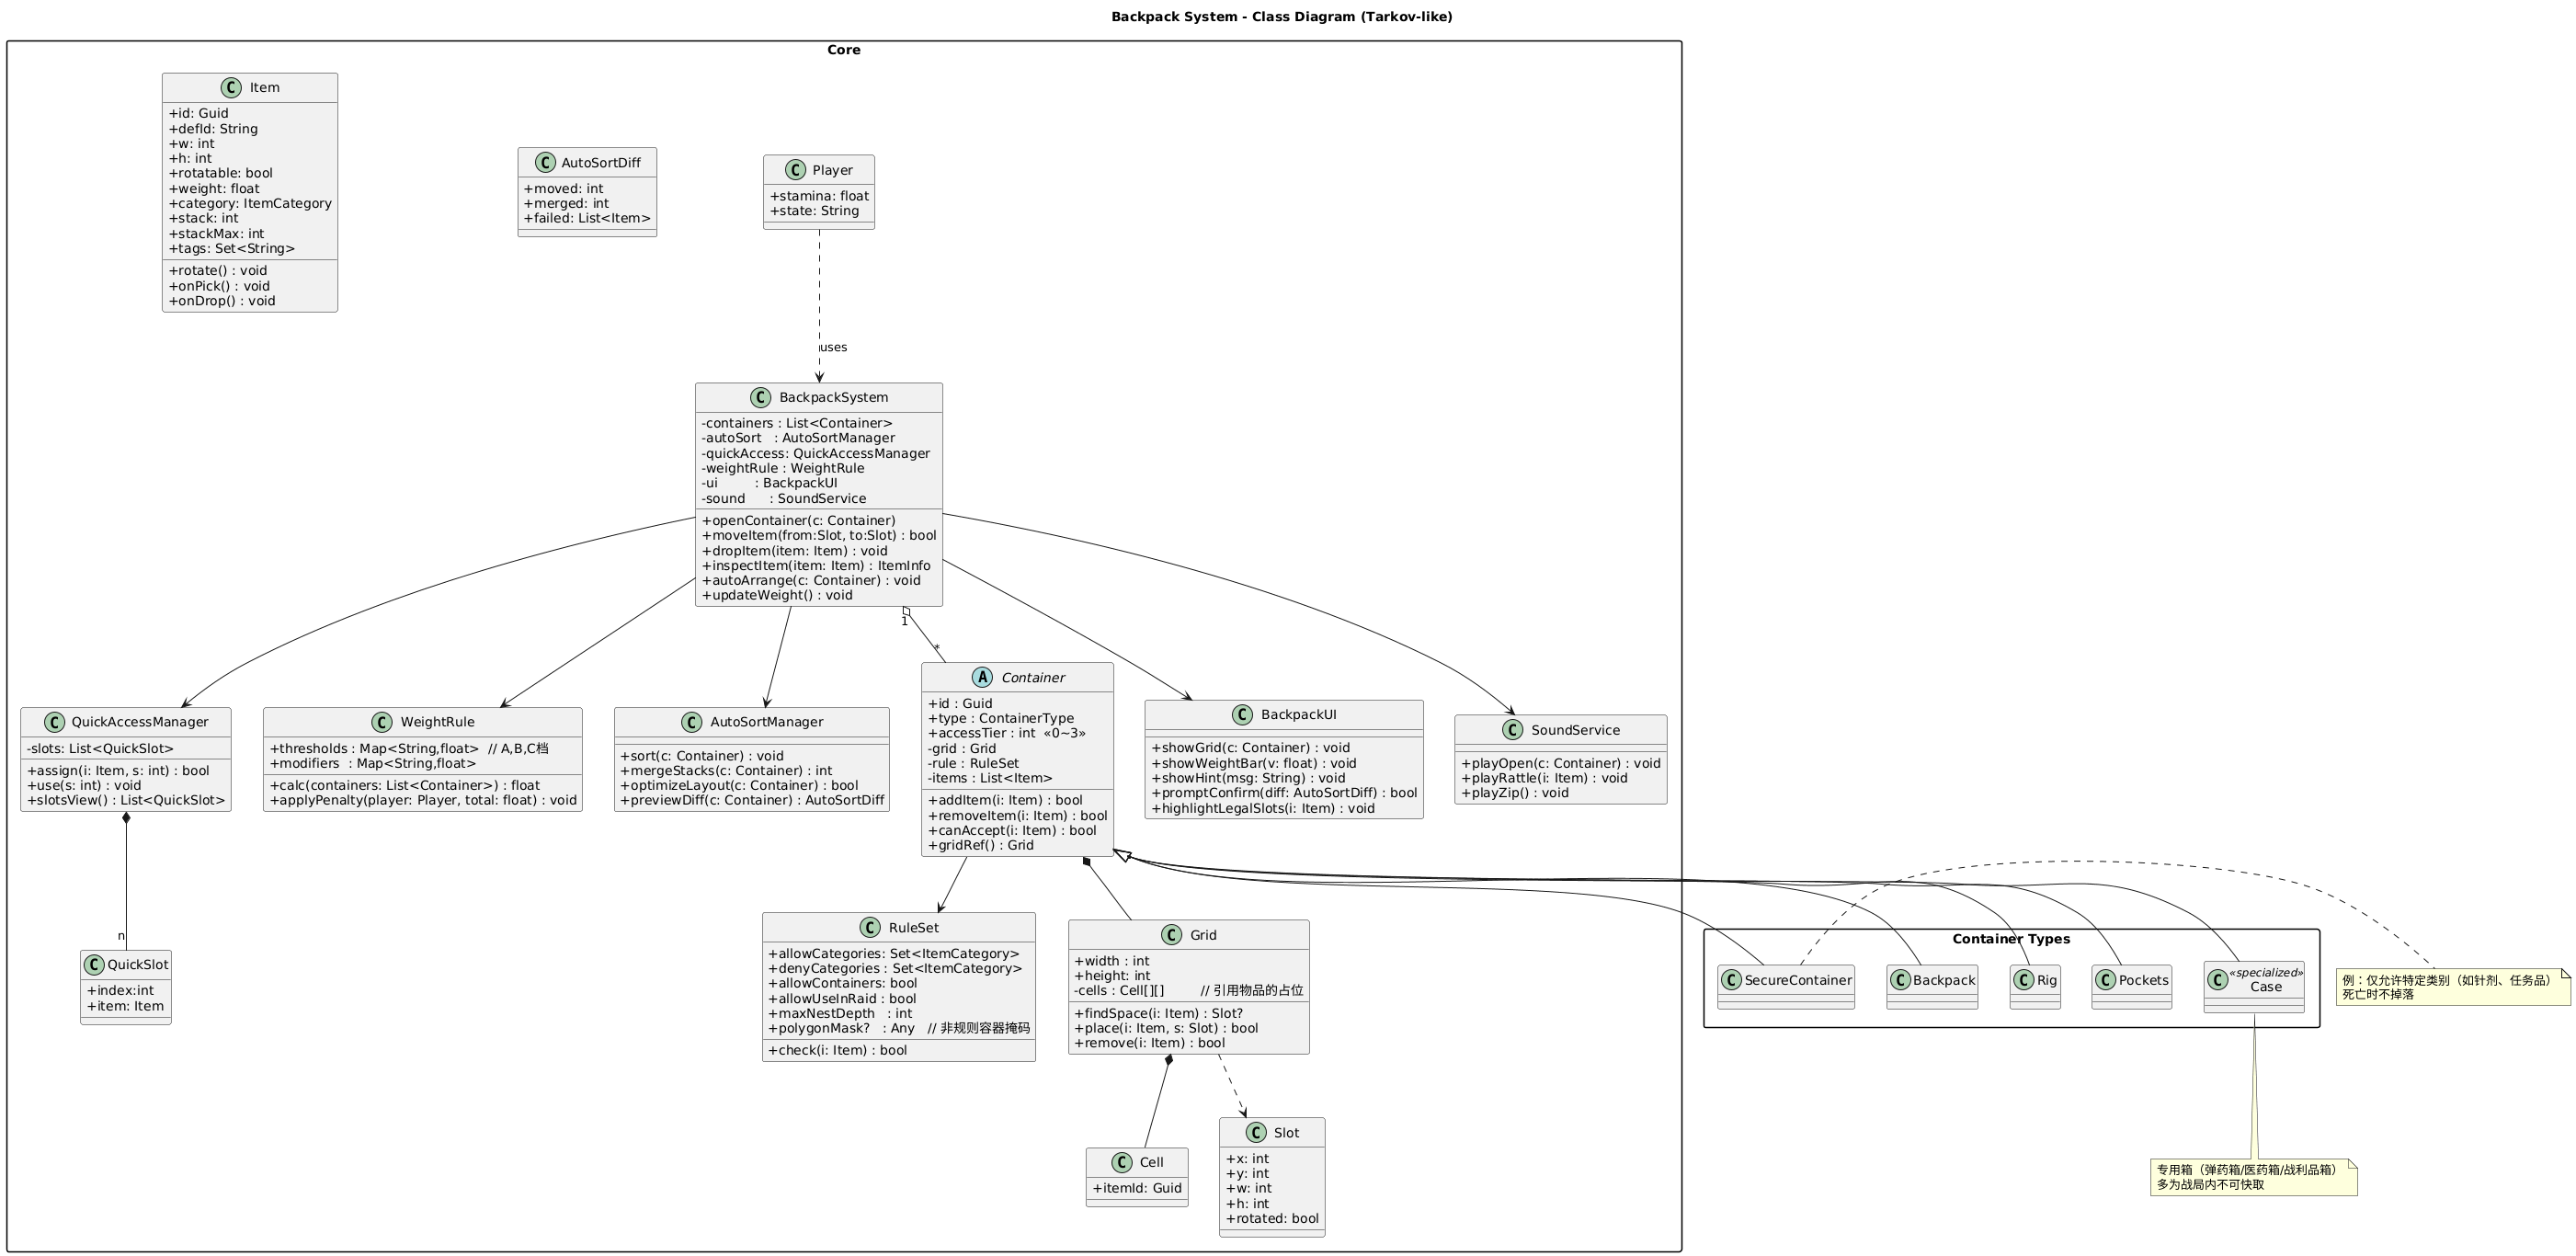
\includegraphics[width=1.5\textwidth]{Fig/UML/Chapter3/3_3_1.png}}
    \caption{物品背包系統類圖}
\end{figure}
\end{landscape}

\begin{landscape}
\begin{figure}[htbp]
  \centering
  \vspace*{\fill} 
      \fbox{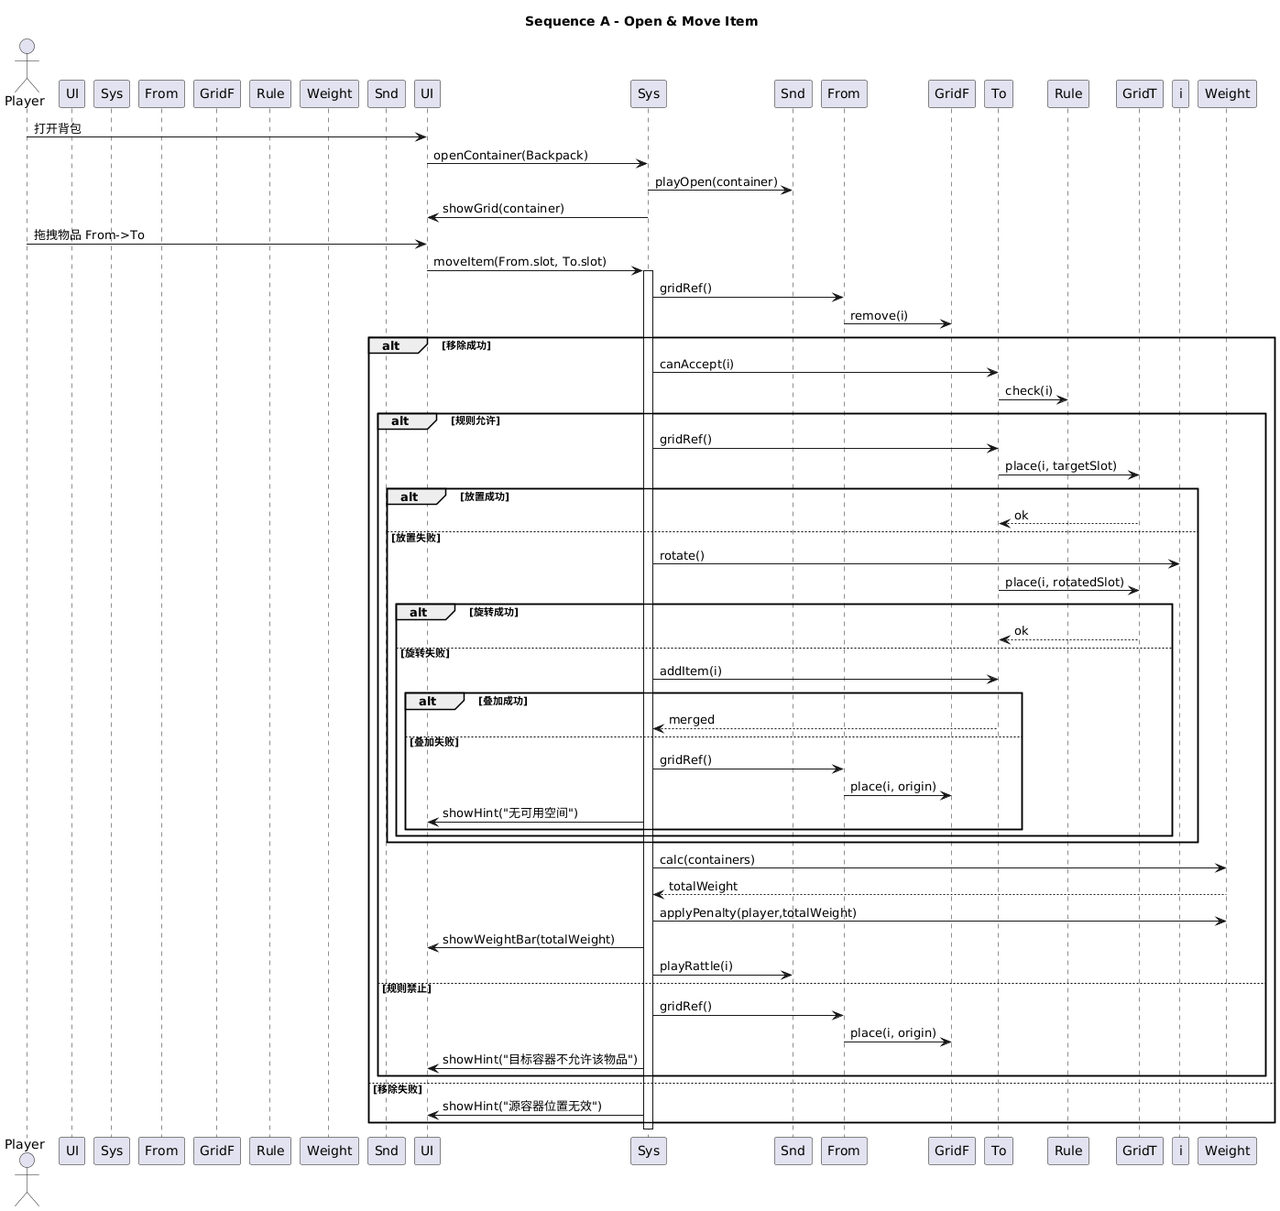
\includegraphics[width=1.1\textwidth]{Fig/UML/Chapter3/3_3_2.png}}
    \caption{移動物品時間序列圖}
\end{figure}
\end{landscape}

\begin{figure}[h]
    \centering
      \fbox{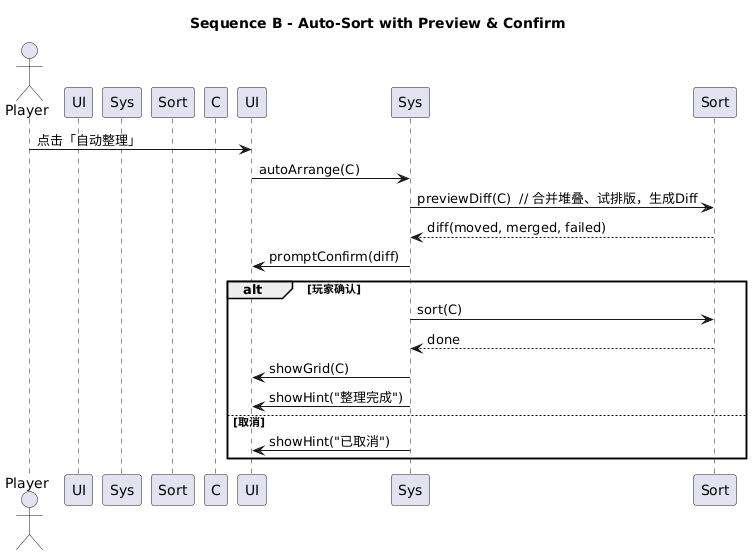
\includegraphics[width=1\textwidth]{Fig/UML/Chapter3/3_3_3.png}}
    \caption{自動整理物品時間序列圖}
    \label{fig:uml-player}
\end{figure}

\subsection{特質系統}

\subsubsection{概述}
玩家分別飾演遊戲中的不同角色，如廚師、醫生、工程師、警衛、搬運工、列車長、商人與獵人。每個角色皆擁有自身的特點與能力，我希望玩家能沉浸於所扮演的角色之中，並完成對應的職責與任務。各種角色的能力以「特質（Trait）」標籤的形式呈現給玩家，使玩家能夠直觀理解角色差異並發展出不同的遊戲策略。

\subsubsection{設計目標}
\paragraph{\Large\bfseries 面向玩家的目標}
\begin{markdown}
- 列車長
  - 擁有列車室銘貼
  - 初始物品：望遠鏡
  - 特質：列車長在駕駛火車時，會消耗更少的煤炭
- 工程師
  - 特質：修復速度更快
  - 特質：製造物品速度更快
- 搬運工
  - 擁有終物倉銘貼
  - 特質：更高的負重能力
  - 特質：更優質的耐力，但代謝較高
- 廚師
  - 擁有火車廚房銘貼
  - 特質：做飯速度很快
  - 特質：代謝較高
- 醫生
  - 擁有火車醫療室銘貼
  - 特質：製造醫療類物品速度更快
  - 特質：製造醫療類物品效用更強
  - 特質：能夠檢查醫療類物品的成分
- 警衛
  - 擁有警衛室銘貼
  - 初始物品：一把左輪手槍、些許子彈
- 獵人
  - 初始物品：一把弓、些許弓箭
  - 特質：使用弓對動物造成更高傷害
- 商人
  - 擁有自己的火車乘客包廂銘貼
  - 特質：檢索容器時，可能會得到更高級的物品
\end{markdown}
\paragraph{\Large\bfseries 面向程序員的目標}
\begin{markdown}
- 獨立系統
- 可拓展新特質，數據驅動
- 統一作用方式：一切特質都轉成對屬性與系統的修飾器（Modifier）／效果（Effect）
- 動態生命週期：開局授予、任務獲得、病理觸發、時效結束
- 網絡與存檔：服務器權威；複製 Trait 列表與活動修飾器；可存檔
\end{markdown}
\paragraph{\Large\bfseries 面向遊戲設計師的目標}
\begin{markdown}
- 策劃透過 CSV 文件去調整特質的數值變化即可
\end{markdown}

\paragraph{\Large\bfseries 特質頭腦風暴}
\begin{longtable}{p{3cm}p{12cm}}
\caption{角色特質系統表（Trait System）} \label{tab:traits} \\
\toprule
\textbf{特質名稱} & \textbf{效果說明} \\
\midrule
\endfirsthead

\multicolumn{2}{c}{{\bfseries 表 \thetable{}（續）}} \\
\toprule
\textbf{特質名稱} & \textbf{效果說明} \\
\midrule
\endhead

\bottomrule
\multicolumn{2}{r}{（未完，續下頁）} \\
\endfoot

\bottomrule
\endlastfoot

% --- 體能相關 ---
\multicolumn{2}{l}{\textbf{體能相關}} \\[3pt]
鐵肺 & 衝刺／攀爬耐力消耗 −20\%，恢復 +10\%。 \\
短氣 & 衝刺耐力消耗 +25\%，恢復 −15\%。 \\
負重猛士 & 負重上限 +30\%，負重懲罰閾值提高。 \\
脆弱後背 & 負重上限 −25\%，超載時更易受傷。 \\
疾跑者 & 基礎移動／衝刺速度 +6\%，起步更快。 \\
跛行舊傷 & 基礎移動速度 −6\%，受傷後額外 −5\%。 \\[5pt]

% --- 代謝與身體狀態 ---
\multicolumn{2}{l}{\textbf{代謝與身體狀態}} \\[3pt]
快速代謝 & 飢餓／口渴衰減 +20\%，食物／水恢復效果 +25\%。 \\
遲緩代謝 & 飢渴衰減 −20\%，進食效果延遲。 \\
快速癒合 & 自然恢復 +40\%，包紮效率 +20\%。 \\
慢性出血 & 流血量 +20\%，包紮需更多材料。 \\
抗毒體質 & 食物／氣體毒素時效 −30\%。 \\
易毒體質 & 食物／氣體毒素時效 +30\%。 \\[5pt]

% --- 精神與情緒 ---
\multicolumn{2}{l}{\textbf{精神與情緒}} \\[3pt]
穩心（抗抖） & 武器／針劑手抖 −30\%，開鏡晃動減小。 \\
硬漢（痛閾高） & 受傷時更不易進入恐慌情緒狀態。 \\
冷靜自持 & 更容易維持冷靜情緒狀態。 \\
易焦慮 & 恐慌累積 +25\%，聽到警報時更易崩潰。 \\[5pt]

% --- 感官與潛行 ---
\multicolumn{2}{l}{\textbf{感官與潛行}} \\[3pt]
輕步如貓 & 移動噪音 −20\%，開關門聲音更小。 \\
腳重 & 移動噪音 +25\%，開關門更響。 \\
夜視尚可 & 黑暗可見度提升（UI／後處理效果），但對眩光更敏感。 \\
順風耳 & 聲源定位更精準（UI提示範圍更大／持續更久）。 \\[5pt]

% --- 技巧與專業 ---
\multicolumn{2}{l}{\textbf{技巧與專業}} \\[3pt]
靈巧指尖 & 開鎖／拆雷／縫合速度 +20\%。 \\
麻醉師 & 針劑持續時間更穩定。 \\
恢復體質 & 使用醫療物品時恢復血量更多。 \\
鑰匙大師 & 車廂／櫃鎖開鎖速度更快。 \\[5pt]

% --- 成癮與物質相關 ---
\multicolumn{2}{l}{\textbf{成癮與物質相關}} \\[3pt]
酒量好 & 酒精增益時長 +50\%，負面效果較輕。 \\
酒精不耐 & 酒精負面效果更強，短暫視野晃動。 \\
煙癮 & 吸煙時增益更強，但戒斷時負面更重。 \\
酒癮 & 飲酒時增益更強，但戒斷時負面更重。 \\

\end{longtable}

\subsubsection{UML圖繪製}

\begin{landscape}
\begin{figure}[htbp]
  \centering
  \vspace*{\fill} 
      \fbox{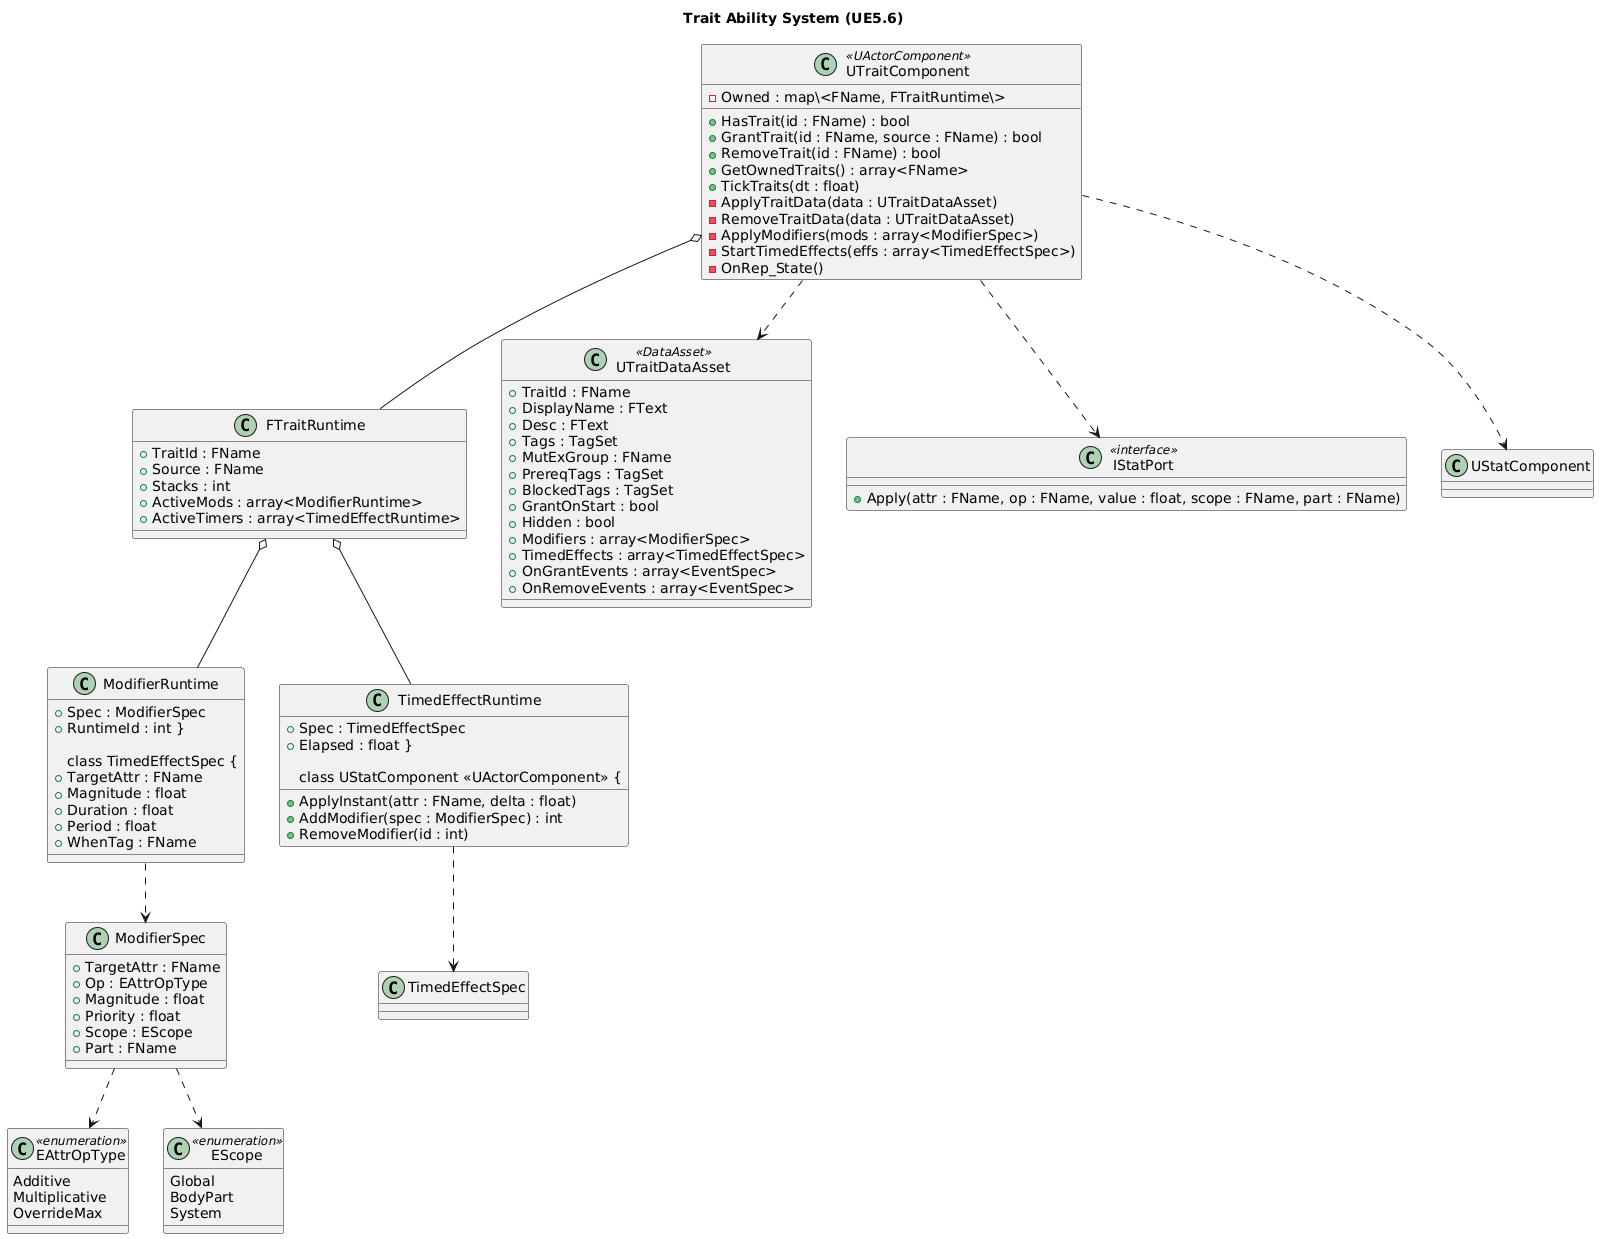
\includegraphics[width=1.24\textwidth]{Fig/UML/Chapter3/3_4_1.png}}
    \caption{特質能力系統類圖}
\end{figure}
\end{landscape}

\begin{figure}[h]
    \centering
      \fbox{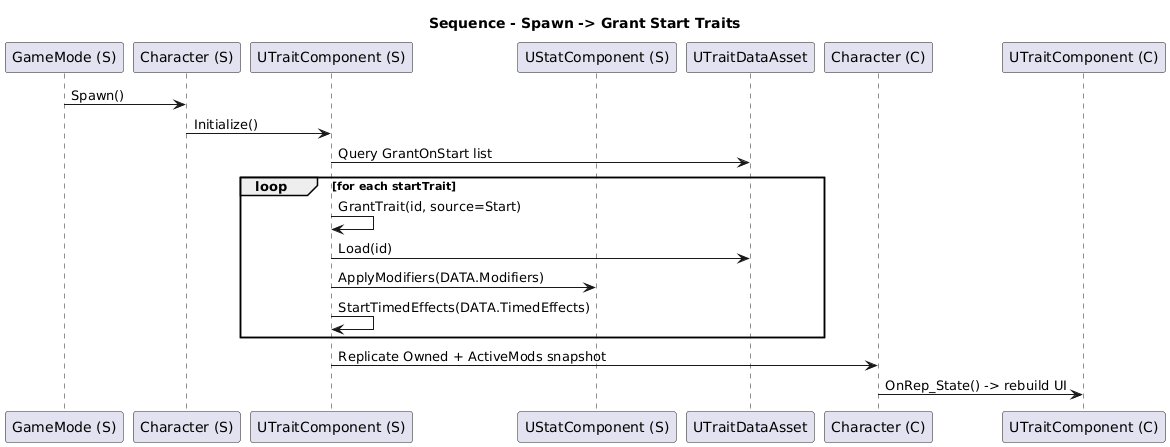
\includegraphics[width=1\textwidth]{Fig/UML/Chapter3/3_4_2.png}}
    \caption{開局時角色特質時間序列圖}
    \label{fig:uml-player}
\end{figure}

\begin{figure}[h]
    \centering
      \fbox{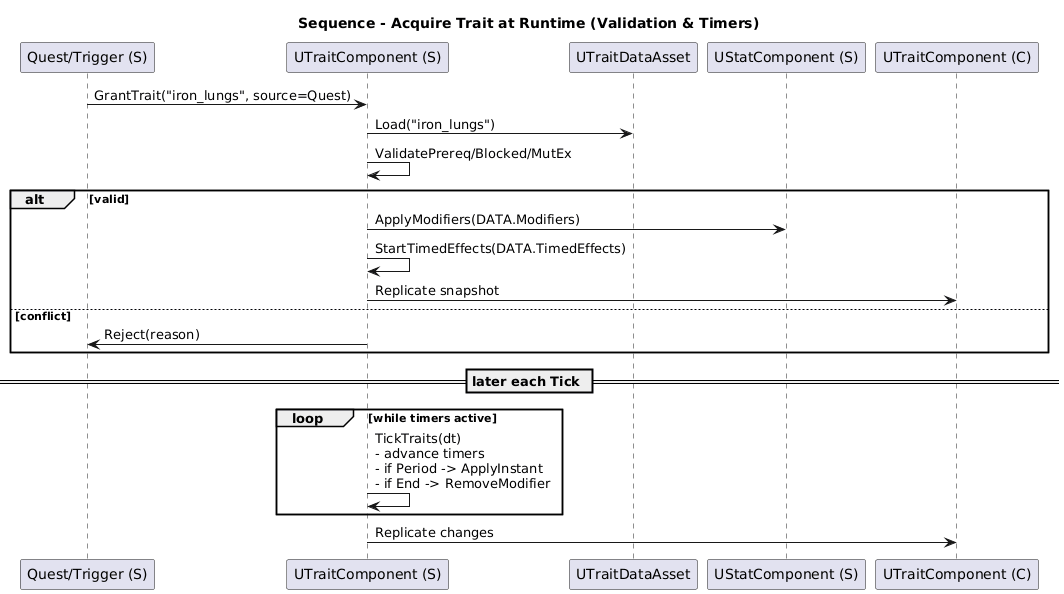
\includegraphics[width=1\textwidth]{Fig/UML/Chapter3/3_4_3.png}}
    \caption{運行時角色特質時間序列圖}
    \label{fig:uml-player}
\end{figure}

\section{火車載體系統}
\subsubsection{概述}
火車不僅僅是一個載具，更是一個多名玩家共同上演戲劇的「舞臺」。
在這列火車上，玩家們需要**生存、工作、合作，甚至彼此勾心鬥角**。
如何合理地設計火車這個載體空間，是整體遊戲機制中極具挑戰性的核心問題之一。

火車同時也是一個**生命系統（Living System）**。
正面陣營的玩家需要維持火車的正常運行，包括能源供應、機械維護、環境控制與資源管理；
而反面陣營則需在暗中製造混亂，通過破壞、干擾、欺騙或奪取控制權，盡可能阻止火車前進。

這樣的設計使火車不再只是背景場景，而是一個會「呼吸」的生態載體：
它連接了玩家之間的合作與對抗，也象徵著整個遊戲世界的運轉與命運。

\subsubsection{設計目標}
\paragraph{\Large\bfseries 面向玩家的目標}
\begin{markdown}
- 列車車頭
    - 鍋爐煤艙
        - 玩家需要不時地填入煤炭資源以讓火車繼續推進
        - 玩家需要清理煤渣，如果在下次點火前有煤渣，則會一段時間後鍋爐爆炸
        - 煤渣會在燒煤後，自動積壓在煤艙的底內
    - 水泵系統
        - 如果在燒煤的過程中，水含量過少，則會炸爐
        - 水位倉
    - 火車控制系統
        - 方向杆
        - 壓力計
        - 剎車杆
        - 節流杆
        - 點火系統
    - 輸煤管道
    - 玩家出生點
        - 車頭控制臺銘貼
        - 望遠鏡
        - 車頂入口（只能進不能出）
    - 輸入水管道
- 煤車車廂
  - 上層煤倉區域
  - 下層儲水區域
  - 玩家出生點
    - 斧頭
    - 煤倉車廂銘貼
  - 車廂末部入口（只能進不能出）
  - 普通工作台
- 餐車車廂
  - 廚房區域
    - 大型爐灶工作台
    - 儲物櫃
    - 裝飾類物品
    - 玩家出生點
    - 車廂頭部入口（只能進不能出）
  - 就餐區域
    - 桌子、椅子
    - 儲物櫃
    - 裝飾類物品
    - 普通工作台
  - 吧台區域
    - 儲物櫃
    - 裝飾類物品
    - 冰櫃
- 醫療車廂
  - 玩家出生點
  - 車廂頂部入口（只能進不能出）
  - 醫療救治公共區域
    - 床
    - 儲物櫃
    - 普通工作台
  - 醫生辦公室
    - 儲物櫃
    - 醫療工作台
    - 小型爐灶工作台
- 乘客車廂
  - 玩家出生點（商人）
    - 商人包廂銘貼
    - 車廂頂部入口（只能進不能出）
  - 乘客包廂（數個）
    - 行李櫃
    - 普通工作台
- 貨運車廂
  - 玩家出生點（搬運工）
    - 貨運車廂內一容器銘貼
    - 斧子
  - 玩家出生點（警衛）
    - 貨運車廂內一容器銘貼
    - 一把手槍
  - 車廂頂部入口（只能進不能出）
  - 儲物櫃
\end{markdown}
\paragraph{\Large\bfseries 面向藝術家的目標}
\begin{markdown}
- 設計火車 2D 平面圖
- 製作火車 3D 模型
- 燈光布置
\end{markdown}
\paragraph{\Large\bfseries 面向程序員的目標}
\begin{markdown}
- 可移動的火車系統
- 物品互動系統
    - 儲物類
      - 額外的背包系統
    - 工作台類
      - 額外的背包系統
      - 物品生成系統
- 門交互系統
    - 開鎖功能
    - 上鎖功能
    - 撬鎖功能
    - 觸發功能
    - 修復鎖功能
\end{markdown}

\section{生態系統}
\subsection{時間系統}
\subsubsection{概述}
本遊戲中，每一局（Round）定義為持續 N 分鐘 的實際遊玩時間；
而在這段有限的現實時間內，遊戲內的世界時間將經歷 M 天 的時間流逝。

時間膨脹的具體計算方式如下所示：
\begin{table}[h!]
\centering
\caption{遊戲時間符號與含義對照表}
\begin{tabular}{|c|l|}
\hline
\textbf{符號} & \textbf{含義} \\ \hline
N & 一局遊戲的現實時長（分鐘） \\ \hline
M & 一局遊戲中經過的遊戲內天數 \\ \hline
D(real) & 現實時間（秒） \\ \hline
D(game) & 遊戲內時間（秒） \\ \hline
T(day) & 遊戲內“一天”所對應的現實時間（秒） \\ \hline
Scale & 時間膨脹比例（遊戲內秒 / 現實秒） \\ \hline
\end{tabular}
\end{table}
在本系統中，定義：
\[
N \text{ 分鐘現實時間} = M \text{ 天遊戲時間}
\]

由於：
\[
1 \text{ day} = 24 \times 60 \times 60 = 86400 \text{ 秒（遊戲內時間）}
\]

則膨脹比例（Scale）可表示為：
\[
\text{Scale} = \frac{M \times 86400}{N \times 60}
\]

因此，對應關係為：
\[
1 \text{ 秒（現實時間）} \rightarrow \text{Scale} \text{ 秒（遊戲內時間）}
\]

換言之，遊戲內時間的流逝速度為現實時間的：
\[
\text{Scale 倍}
\]

\subsubsection{設計目標}
\paragraph{\Large\bfseries 面向玩家的目標}
\begin{markdown}
- 讓玩家體驗白天與黑夜的交替，類似於現實生活中的節奏與感受。
\end{markdown}

\paragraph{\Large\bfseries 面向遊戲設計師的目標}
\begin{markdown}
- 策劃可以自由調整時間膨脹比例以更新玩家體驗
\end{markdown}


\subsubsection{UML圖繪製}
\begin{landscape}
\begin{figure}[htbp]
  \centering
  \vspace*{\fill} 
      \fbox{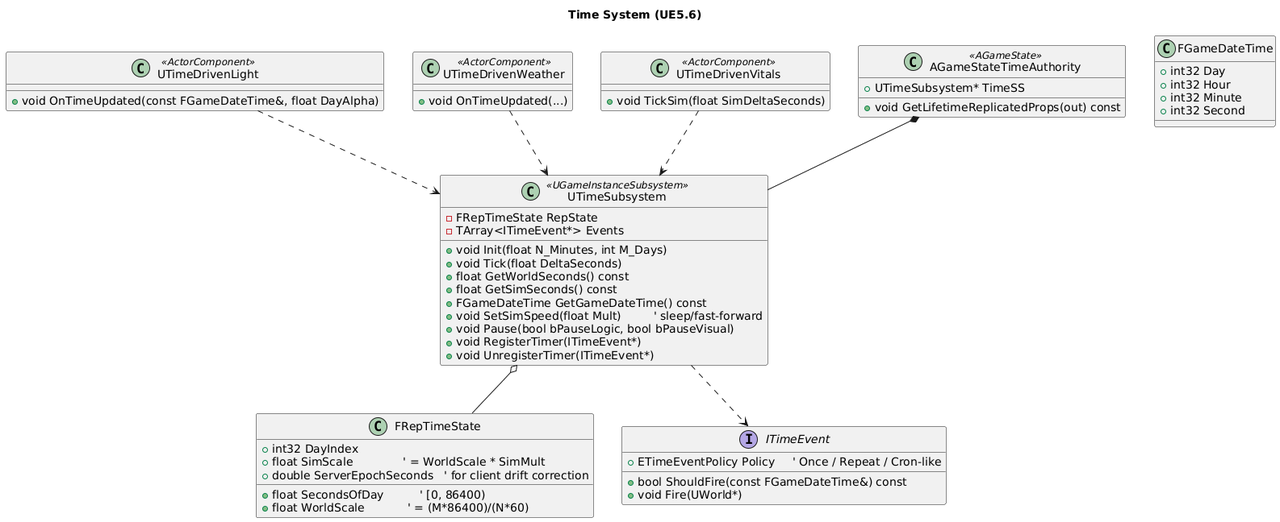
\includegraphics[width=1.5\textwidth]{Fig/UML/Chapter3/3_5_1.png}}
    \caption{時間系統系統類圖}
\end{figure}
\end{landscape}

\subsection{AI系統}
\subsubsection{概述}
遊戲世界中的生物 AI 具有多樣的作用與功能，如何構建一個兼具樂趣與挑戰性的 AI 系統，是不可避免的設計課題。

一般而言，高危險度的 AI 意味著高報酬，而攻擊性較低的 AI 則對應較低的回報。例如：

* 食草類生物 AI 通常位於生態鏈的被掠食者地位，玩家可使用工具進行狩獵與採集；
* 食肉類生物 AI 則多具主動攻擊性，會對玩家構成威脅，迫使玩家制定防禦或迴避策略。

此外，控制不同物種之間的關係（如掠食與共生）、模擬生物群落分佈與遷移行為，也是生態系統設計中的重要環節。
這不僅影響玩家的探索體驗，也直接關聯到資源循環、環境平衡與遊戲世界的生命力呈現。

\subsubsection{設計目標}
\paragraph{\Large\bfseries 面向玩家的目標}
\begin{markdown}
- 無攻擊性 AI
  - 依環境而定
- 攻擊性 AI
  - 依環境而定
- 交易型 AI
  - 可以以物換物
\end{markdown}
\paragraph{\Large\bfseries 面向藝術家的目標}
\begin{markdown}
- 3D 模型資產
- AI 行為動畫
\end{markdown}
\paragraph{\Large\bfseries 面向程序員的目標}
\begin{markdown}
- 架構分層
  - 控制全身生態預算、季節/天氣修正、各生物群落的上限與更新頻率。
  - 定義體型、移動、感知、性情、群居測則、家域半徑、食性標籤等（數據驅動）。
  - 行為樹 + 黑板 + 感知組件，內含**生命特徵/情緒**（饑餓、體溫、恐懼、慾望、體力）**與物種特技**。
- 關鍵數據與驅動
  - Biome/Spawn 表（CSV/DataTable）：決定不同地帶“物種—數量範圍—成群機率—刷新間隔—地形標籤”。
  - Species DataAsset：物種屬性參數（感知、速度、攻擊性、成長傾好、行為特技）。
  - 所有關聯行為伺服可隨變化更新，策劃可熱更新。
- 生成與回收（Spawner）
  - 基於 Biome 的數組刷附（領域個體 + 若干隨機），距離玩家 150~250m 外生成，>400m 回收。
  - PopulationCap 限制併發數量，Respawn 在玩家離開與冷卻後才啟動，避免“刷臉感”。
  - 夜間/季節可對數量與攻性加成，形成節奏變化。
\end{markdown}
\paragraph{\Large\bfseries 面向遊戲設計師的目標}
\begin{markdown}
- AI數值的調參
- 群路分佈的設計
\end{markdown}
\subsubsection{UML圖繪製}
\begin{landscape}
\begin{figure}[htbp]
  \centering
  \vspace*{\fill} 
      \fbox{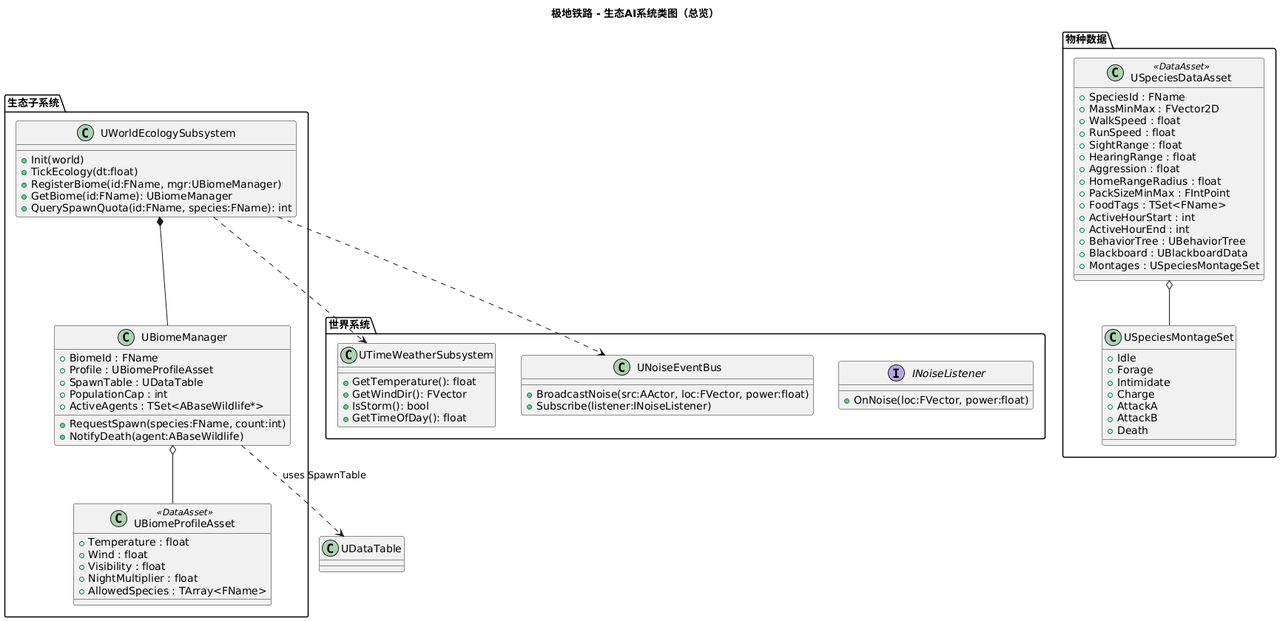
\includegraphics[width=1.5\textwidth]{Fig/UML/Chapter3/3_6_1.png}}
    \caption{生態AI系統類圖}
\end{figure}
\end{landscape}

\subsection{環境系統}





\section{物品系統}
\subsubsection{概述}
\subsubsection{設計目標}
\paragraph{\Large\bfseries 面向玩家的目標}
\begin{markdown}

\end{markdown}
\paragraph{\Large\bfseries 面向藝術家的目標}
\begin{markdown}

\end{markdown}
\paragraph{\Large\bfseries 面向程序員的目標}
\begin{markdown}

\end{markdown}
\paragraph{\Large\bfseries 面向遊戲設計師的目標}
\begin{markdown}

\end{markdown}
\subsubsection{UML圖繪製}



\citep{abdoh2019} 引用
\subsection{論文寫作依據}
正文部位写
\chapter{美術與關卡設計}
\section{美術風格}
\section{關卡設計}
\citep{abdoh2019} 引用
\subsection{論文寫作依據}
正文部位写
\chapter{結論與建議}

\citep{abdoh2019} 引用
\subsection{論文寫作依據}
正文部位写
\chapter{未來工作}
\section{項目的完成度}
\section{利潤與規劃設計}
\citep{abdoh2019} 引用
\subsection{論文寫作依據}
正文部位写


% 導入參考文獻,請檢查項目中是否存在 bbl 格式文件
% 若無, 請用chrome 應用插件 overlear texAide 對 bib 文件進行格式轉換; 
% 注意:下面的命令參數為不帶後綴的文件名, 
\addreference{ref}

% 導入附錄文件
\input{content/d_appendix}


% 導入致謝頁面
\input{content/e_ack}


% 導入個人簡歷
\input{content/f_cv}



\end{document}